\documentclass[class=article,crop=false,11pt]{standalone}

\usepackage{../setting/preamble_}

\begin{document}
\twocolumn

\section{Methodology}
\subsection{Preliminary Analysis}
At an earlier stage of the project, we plan to build an octave piano with twelve notes including minor keys. At that stage, we analyzed the frequency spectrum of each note and found out it is possible to produce a majority feeling of sound with only four harmonics to a given note.
\par
After synthesizing all the keynotes from its harmonics using Matlab, we moved to circuit development. At this stage, we decided to stimulate only one note from the piano because the generation of notes is modularizable. For this purpose, we have chosen the C-wave which is in the middle of the spectrum.
\begin{figure}
    \begin{subfigure}{.45\columnwidth}
        \centering
        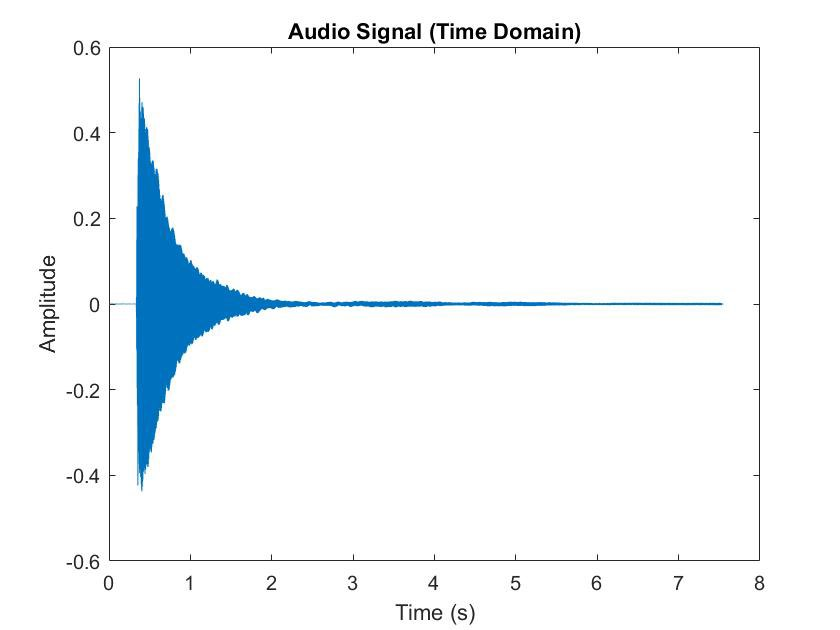
\includegraphics[width=.9\columnwidth]{c_wave}
    \end{subfigure}
    \begin{subfigure}{.45\columnwidth}
        \centering
        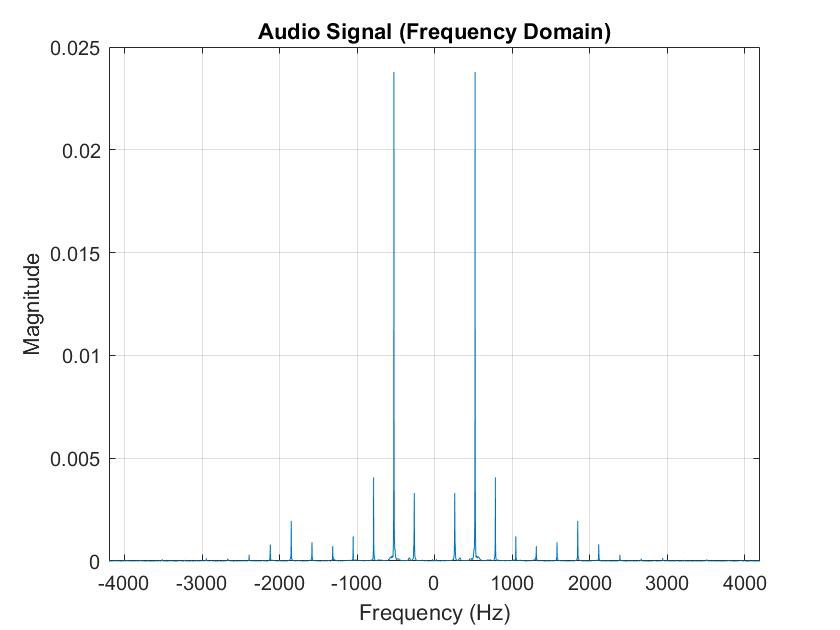
\includegraphics[width=.9\columnwidth]{spectrum_c}
    \end{subfigure}

\end{figure}
\subsection{Circuit Design}

\begin{figure}
    \begin{center}
        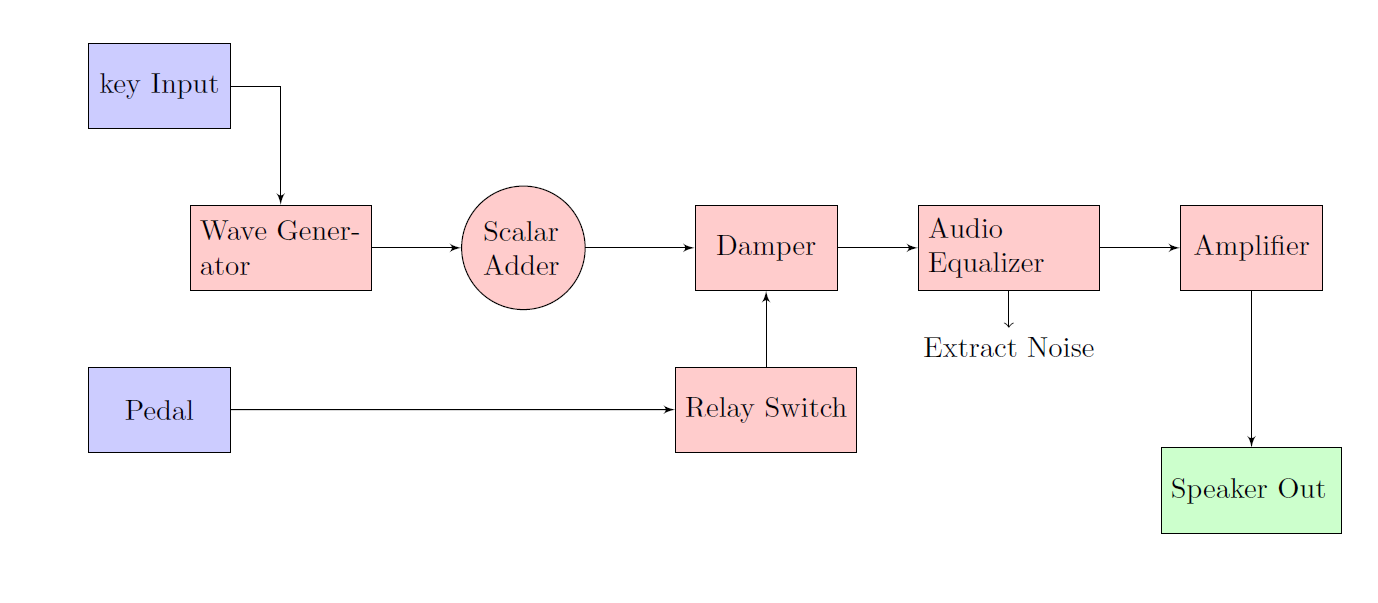
\includegraphics[width=\columnwidth]{flow}
        \caption*{Block Diagram of the Circuit}
    \end{center}
\end{figure}
\subsubsection{Wave Generator}
Square wave generation of half the frequency together with a bandpass active filter is considered in the first stage of the circuit development. Need for achieving a larger Q factor for the filter as the number of harmonics increases, lift the choice to not-feasible.
\par
Moving towards a stable solution brought the Wien bridge oscillator into play. These oscillators have the flexibility over frequency choice ($\frac{1}{2\pi RC}$) making them the most suitable option to be used with modularizable piano.
\subsubsection{Key and Pedal}
\subsubsection{Scalar Adder}
\subsubsection{Amplifier}
At earlier stages, the amplifier was implemented in class-A configuration. The requirement for lower output resistance of the bias path leads to high power dissipation in the signal-free state. This made such a model impossible without larger heatsinks at the cost of low power efficiency.
\begin{figure}
    \begin{center}
        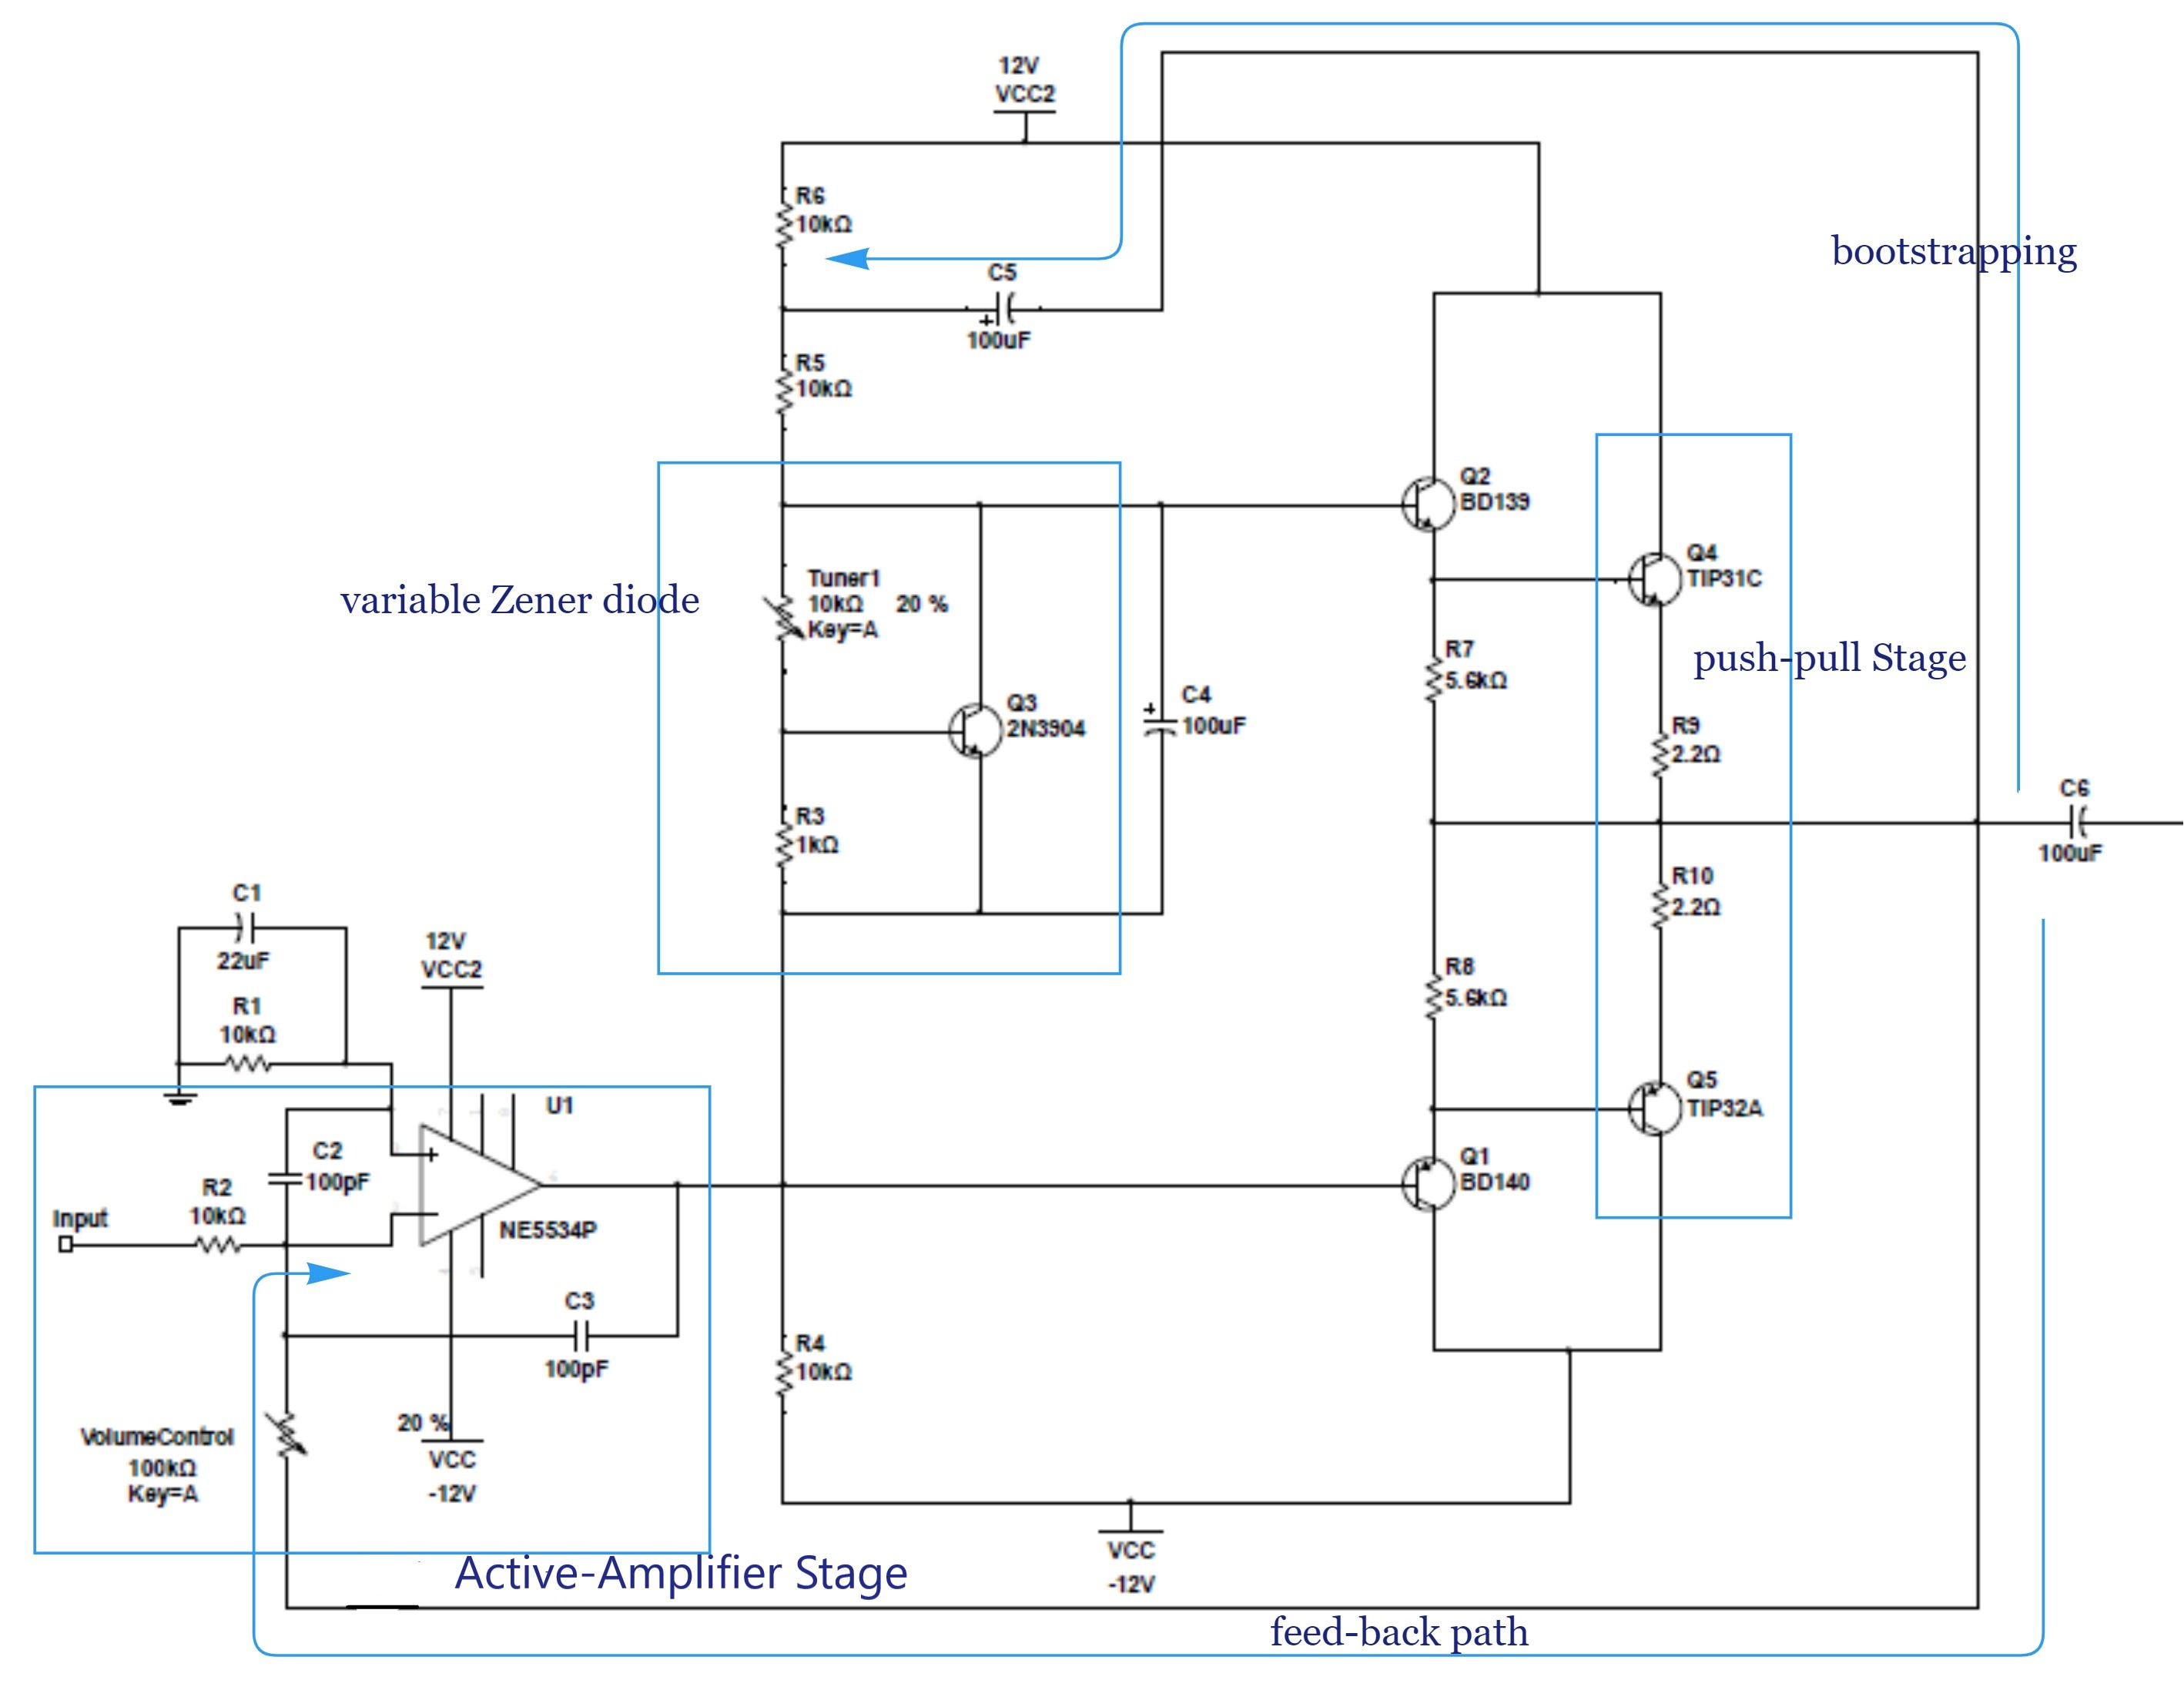
\includegraphics[width=\columnwidth]{amplifier_cd}
    \end{center}
\end{figure}

\textbf{Active Amplifier Stage}: In the first stage of the amplifier an op-amp is used in the inverting-amplifier configuration. The feedback path is connected to the end of the overall circuit to ensure enough current supply available in the output. The op-amp NE5534 was chosen for the purpose according to its key characteristics such as high unity-gain bandwidth(10MHz), low harmonic distortion, and high common-mode rejection ratio (100dB). The values of C2 and C3 are chosen to allow only higher frequencies($>20kHz$) to pass through. These are utilized in a manner to remove high-frequency noises from the wave-form.
\\
\textbf{Push-Pull Stage}: Considering the requirement of high power gain it is decided to engage Darlington pairs for this purpose. These components failed in the long run due to the inability of compensating for high power dissipation. Considering this, the design moved to engage two coupled BJTs to allow the choices for transistors to be used in the high current path. The similar pairs TIP31C and TIP32C were chosen after considering their high power compensation capability(around 40W).
\\
\textbf{Bias}: Due to the requirement for a sudden supply of high current on the keypress, the signal gets noisy when we drive the speaker without any bias. In earlier stages, a few diodes are used to bias the circuit which failed to get rid of the noise. As the next step, we used Zener diodes that provide the capability to choose higher bias voltage. This results in the low efficiency of the circuit.
After considering all the methods it is decided to implement the variable Zener diode which has the flexibility over varying bias voltage in a wider range. This provides control over two extremities, effecieny and quality of the output.
\\
\textbf{Bootstrapping}: The capacitor C5 gets charged to the pre-decided bias voltage.  By maintaining the circuit time constant very large ($t=R5\parallel R6\star C5>0.5S$) the overall bias voltage of the circuit is maintained as a constant value to compensate for the effect of thermal runaway.
\end{document}